
\section{Problem Formulation}
\label{sec:ProblemFormulation}


\subsection{Node Fault Graph}
\subsubsection{Node Fault tolerant (NFT)}
We refer to the concept of $k$-NFT\cite{harary1996node}. Let $G(V,E)$ be a graph with $n$ nodes and $q$ edges. An $(n+k)$-node graph $G^*$ is k-node fault-tolerant, or $k$-NFT, with respect to $G$ if every graph $G^*-R$ obtained by removing any nodes set $R$ of $k>0$ nodes from $G^*$ contains $G$. Generally speaking, $G$ is subgraph isomorphism of $G^*-R$. We will refer to $G^*$ as a $k$-NFT supergraphs of $G$ or simply as a $k$-NFT($G$). We also say $G^*\cong$ $k$-NFT($G$), the set of all k-NFT($G$) supergraphs of $G$.

The complete graph $K_{n+k}$ of $n + k$ nodes is trivially a k-NFT supergraph of every $G$ that contains up to n nodes. We are concerned mainly with $k$-NFT graphs that satisfy the following optimality criterion: If $G^*$ has the smallest number $|E(G^*)|$ of edges among all $(n + k)$-node supergraphs that are $k$-NFT with respect to $G$, then $G^*$ is optimally $k$-NFT with respect to $G$. The number $NFT_{ec}$$(G,k)$ =$|E(G^*)-E(G)|$ is called the $k$-NFT edge cost of $G$. The number $NFT_{nc}$$(G,k)$ =$|V(G^*)-V(G)|$ is called the $k$-NFT node cost of $G$, however $NFT_{nc}$$(G,k)$ = k with respect with k node fault tolerant graph of graph $G$ . For example, $NFT_{nc}$$(C_5,1)$ and $NFT_{ec}$$(C_5,1)$ of graph $C_5$ is 1 and 5 respectively as show in Fig.\ref{fig:NFTexample}.

\begin{figure}
  \centering
  % Requires \usepackage{graphicx}
  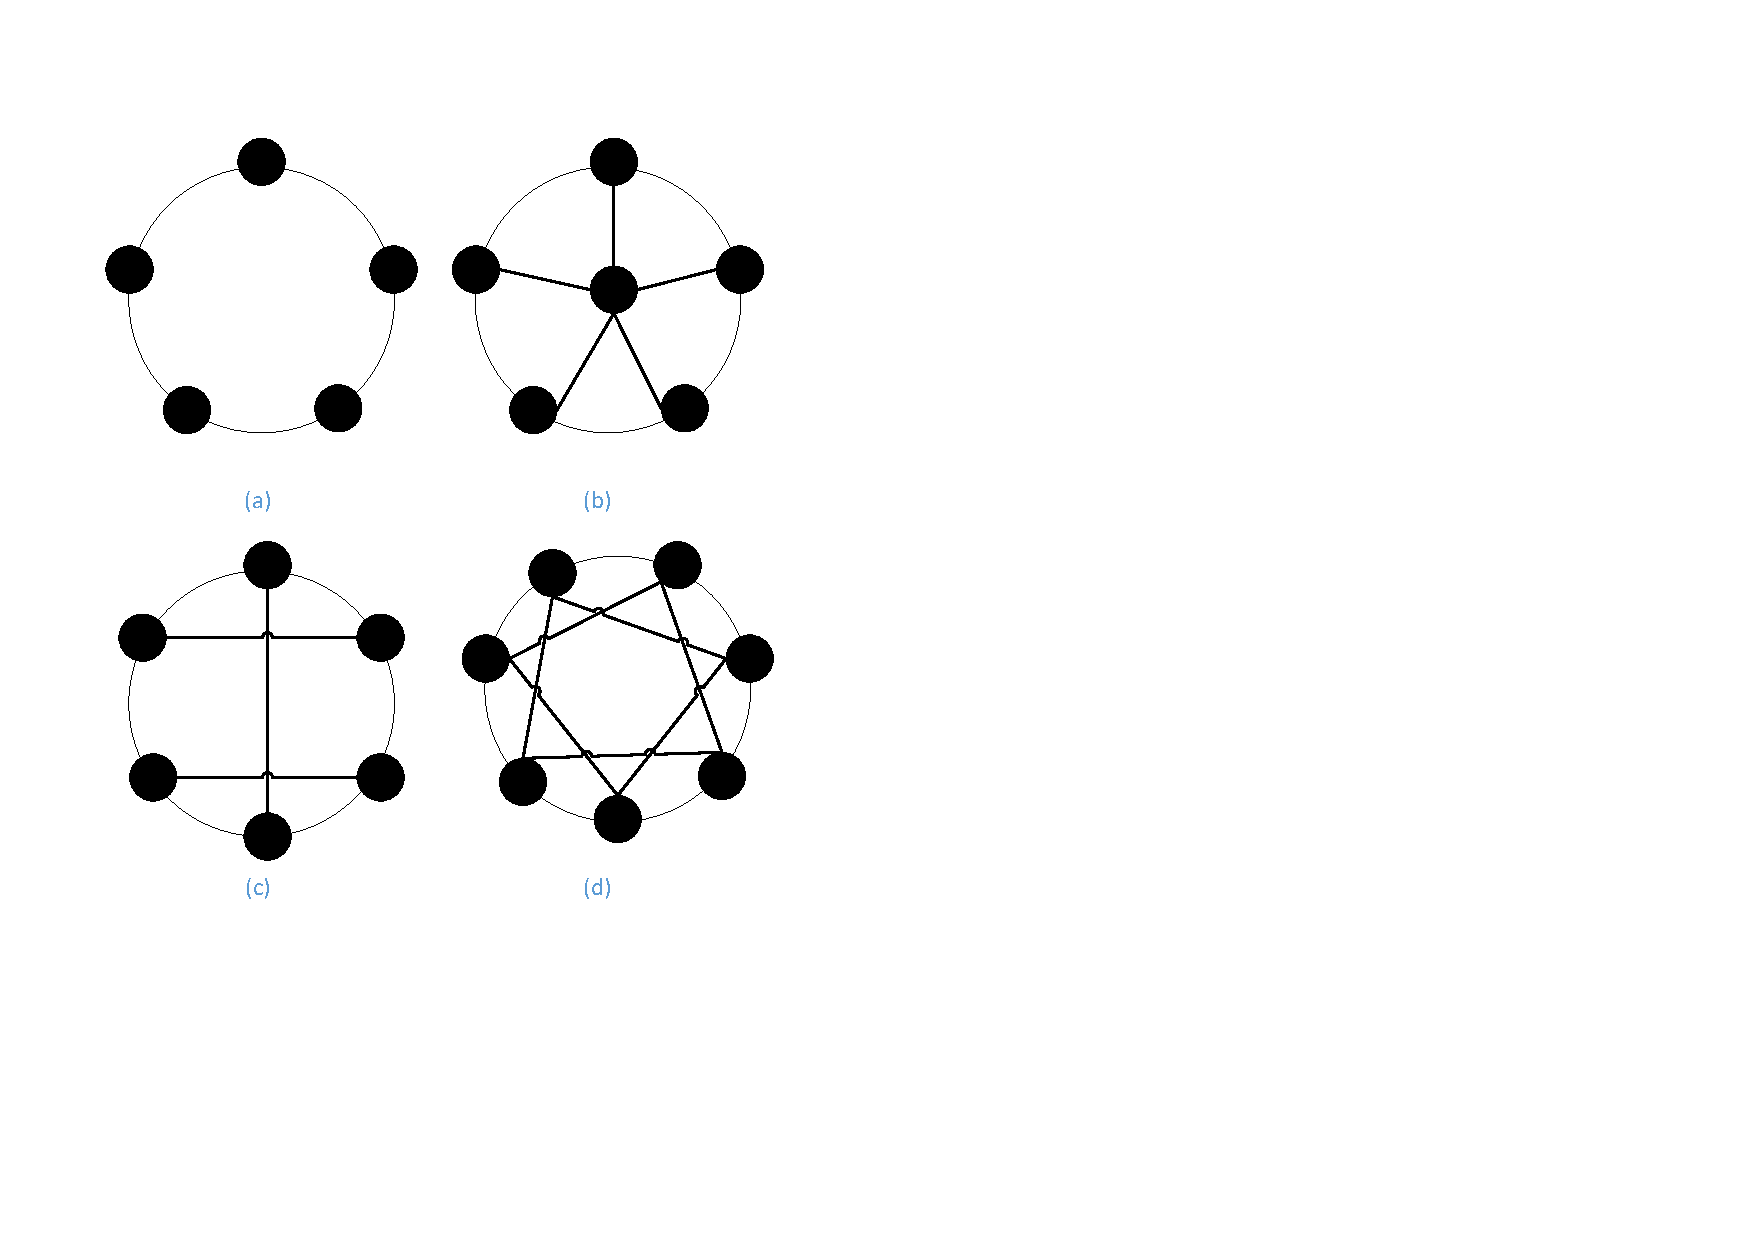
\includegraphics[width=2.5in]{Fig/NFTexample}\\
  \caption{(a)The cycle $C_5$; (b)a nonoptimal $1$-NFT($C_5$), $|R|$=1 ; (c) an optimal $1$-NFT($C_5$), $|R|$=1; (d) an optimal $2$-NFT($C_5$),$|R|$=1 }\label{fig:NFTexample}
\end{figure}

\subsubsection{Service Node Fault Tolerant (SNFT)}
When every nodes of graph $G(V,E,S)$ have a specific services set $S$ (corresponding to node's service function set) and every nodes is marked by only one service set (every node of virtual network just run only one type of service function), which is denoted by node type. A $(n+k)$-node graph $G^o$ is k-service node fault tolerant, or $k$-SNFT, with respect to $G(V,E,S)$ if every graph $G^o-R$ obtained by removing any nodes set $R$ of $k>0$ nodes from $G^o$ contains $G$, $G$ is subgraph isomorphism of $G^o-R$ and the node service of any nodes $n$ of $G$ belong service set of node $n^o$ corresponding to node $n$. We will refer to $G^o$ as a $k$-SNFT supergraphs of $G$ or simply as a $k$-SNFT($G$). The number $SNFT_{nc}$$(G,k)$ =$|V(G^o)-V(G)|$ is called the $k$-SNFT node cost of $G$. The number $SNFT_{ec}$$(G,k)$ =$|E(G^o)-E(G)|$ is called the $k$-SNFT edge cost of $G$. Suppose every node of added nodes contain all service types in current above definition.
\subsubsection{SNFT with B}
After our simple inference, if we think the node cost $SNFT_{nc}(G,k)$  is more important cost than $SNFT_{ec}(G,k)$  edge cost, moreover the added node $B(V,S)$ could have a service set rather than contain all types of service( every node of substrate network contain various combination of service type), Based real situation that the added node should be limited in specific service set through our analyzing the real-world practical phenomenon.(should cite a paper).

A backup (redundant) node b must not be able to assume full execution of a failed critical node c.

Suppose added nodes as backup node set $B(V,S)$, where every nodes of backup node set $B$ have a service set. The $k$-SNFT($G,B$) is denoted by requesting a k service node fault tolerant graph of graph $G$ and added nodes belong backup nodes set $B$. For example, as shown in Fig.\ref{fig:SNFTBexample}, every backup node have individual service set. In Fig.\ref{fig:SNFToptimal_n1Fail} displaying the transformed graph after node $v_1$ failure.

%The limited node of $G^o-G$ with respect to any $G^o$ is used as inserted node from specific node set $B$ which is premise. k-specific node fault-tolerant graph of $G$ with limit-inserted node set $B$ is denoted by k-SNFT($G,B$).


\subsection{Complexity of Service Node Fault tolerant}
\label{sec:Complexity}
This computation complexity of $k$-SNFT graph problem $k$-SNFT($G(V,E,S)$) is NP, whose proof is below. when just exist one service type in Graph $G$, the problem is degenerated into k-node fault-tolerant graph problem. when Graph $G$ just have one type of service, we must add k backup node and add some edges into graph $G$ to construct $k$-SNFT graph, meantime the simplified problem is of equivalance to problem that k-node fault-tolerant $k$-NFT graph problem , which is proof as NP\cite{harary1996node}.

when added node set is given and confirmed aforehand , $k$-SNFT($G(V,E,S)$) is subproblem of the problem $k$-SNFT($G(V,E,S),B(V,S)$). Therefore, according to  the  reducibility theorem\cite{cormen2009introduction} in computer complexity field, it is easy to conclude that problem $k$-SNFT($G(V,E,S),B(V,S)$) is NP also.

$k$-SNFT($G(V,E)$)$\subset$$k$-SNFT($G(V,E,S)$)$\subset$$k$-SNFT($G(V,E,S),B(V,S)$)

Suppose topological structure of graph $G$ is path $P$, k-SNFT($P(V,E,S),B(V,S)$) is NP, the proof is below, exist one node $v_i(v_i\in V)$ and we add backup nodes and some edges to protect the node $v_i$, the former graph $P$ firstly is changed into $P+n$, nevertheless topological structure of $P+n$ may is not path, or be tree and non-tree graph. then protect other nodes of $V$ except node $v_i$, the problem become $(k-1)$-NFT problem.

Furthermore, deriving optimal graphs G0 with minimal links for any general graph G has exponential complexity. To the best of the authors’ knowledge, optimal solutions are found only on regular graphs such as lines, square-grids, circles, and trees [14, 1, 12].

However, this poses a limitation since the result only guarantees graph isomorphism and not equality.In other words, there may be a need to physically swap remaining VMs while recovering from some failure in order to return to the original infrastructure G. Recovery may then be delayed, or require more resources for such swapping operations.

Minimizing the physical footprint of these redundant links during physical embedding give rise to a tight coupling between the virtual nodes and links.
%the computation complexity of k-SNFT($T(V,E,S),B(V,S)$) is similarly available.

%Edge fault tolerant problem is subgraph of node fault tolerant problem.

%We consider a resource deployment problem in a virtualized network infrastructure, such as a data center, where the virtualized resources can be leased with reliability guarantees. Each resource lease request is modeled as undirected attributed labeled graph $G=(V,E,S,L)$. V is a set of compute nodes, E is a set of edges ,S is a types set of node V service functions and L is label of node.



\subsection{Substrate Network}
Substrate network is referred as Network Functions Virtualization Infrastructure or Physical Network,  We model the Substrate network(SN) as an undirected attributed simple graph $G^S (V^S,E^S,S^S,L^S)$, where $V^S$ and $E^S$ is the set of substrate nodes and substrate links respectively, $S^S$ is the service function set on which substrate nodes can run, $L^S$ is label of substrate nodes. Each substrate node (link) is associated with the residual computing (communication) resource capacity. Each node $v_i$ has an available computational capacity of $c_i$. Each undirected link $e_{ij}$ has an available bandwidth of $b_{ij}$. Furthermore, a dynamic embedding approach is considered in this Sec.\ref{sec:embeddedVirtualNetwork}.

\subsection{Virtual Network Request Model}
A topological graph for a virtual network(VN) request is an undirected attributed labeled graph, denoted as $G^V (V^V,E^V,s^V,L^V)$, where $V^V$ corresponds to a node set, $E^V$ denotes a set of bidirectional edges among the VN nodes and $s^V$ denotes a service type among the VN nodes, $L^V$ denotes node's label. Each task node $v_i^V$ specifies the needed available computational resource $c_i^V$, and each edge $e_{ij}$ specifies the requested amount of communication (bandwidth) resource $b_{ij}^V$ as shown in Fig.\ref{fig:VNQ}


\subsection{Embedded Virtual Network}
\label{sec:embeddedVirtualNetwork}
There exist many approaches is modeled as the VN embedding (VNE) problem which attracts a broad interest recently. VNE is extremely important in order to maximize the number of coexisting VNs and increase the utilization of substrate infrastructures. Most of the proposed approaches decompose the problem into two phases, the node embedding phase and the link embedding phase, to reduce the overall complexity of this problem. When a virtual network request has been inserted in to substrate network, additional information is attached virtual network's node, denote $G^V (V^V,E^V,s^V,L^V,S^V,C^V,B^V,M^V_V)$ as embedded virtual network as shown in Fig.\ref{fig:eVN}. $S^V$ denote a set of service type set $S^V_i$($s^V_i\in S^V_i$) which corresponding to every VN nodes $v_i$. $C^V$ denote node's computational resource's capacity. $B^V$ denote edge's bandwidth resource's capacity.

\subsection{Survivable}
%We define reliability as the probability that critical nodes of a VInf remain in operation, over all possible node failures. This is not to be confused with availability, which is defined as a ratio of uptime to the sum of uptime and downtime

Survivability is guaranteed on the set of critical nodes $C\subset V$ of a VN through redundant virtual nodes with backup nodes set $B(V,S)$. A backup (redundant) node $b_i$ may not be able to assume full execution function of a failed critical node $c_i$. Hence, the backup node may not have sufficient resources in terms of computation resource.


%\subsection{How many backups?}
%The number of backup nodes depend on the physical mapping, and the failure models of both the physical nodes and the virtual infrastructure.

%The problem is to  allocate least resources for a VN $G$, including redundancy such that a reliability guarantee of at least r is achieved.


\subsection{why happen Survivable embeded Virtual Network Request}
The software-defined NFV architecture further offers agile traffic steering and joint optimization of network functions and resources.


%When a survivable request of virtual network is coming, survivable virtual network requests are associated with node's service functions.
In any real virtual networks, any nodes of virtual network  are deployed with a service function and the corresponding physical node could run some various service functions. After virtual network VN is embedded into substrate network, a running node of physical network could fail multiple virtual network so that we should obtain survivable eVN to be embedded into substrate network so that recovery from the failure even though one or multiple nodes of virtual network failed. The added nodes of survivable embedded virtual network are embedded into substrate network ultimately, the added nodes have specific service functions similarly.

\subsection{Survivable embedded Virtual Network Request}

In this section, we define the SeVN design problem as follows: for a given VN request with $|V|$ nodes, the VN is already embedded in substrate network SN and running service $s_i(s_i\in S)$, protect the VN with some additional nodes and a set of appropriate links to connect these nodes, and reserve sufficient computing and communication resources in these nodes and links to guarantee the restorability of VN request after a facility node failure.


There are different combinations of service type among all nodes of virtual network, and there is only one type of service type running on the corresponding virtual node at one moment.

There exist many backup virtual nodes $B(V,S)$ which are abstracted from un-occupied substrate network's node. When one fault node $v_i$ appeared in virtual network request $G(V,E,S,L)$, Solving the survivable request of embedded virtual network is of approximately equivalence with asking 1-SNFT$(G,B)$ of graph $G$ and backup nodes set $B$.

An example of a typical survivable request of embedded virtual network is show in Fig.\ref{fig:VNQ}.

\begin{figure*}[tp]
\centering
\begin{minipage}[t]{0.3\linewidth}
\centering
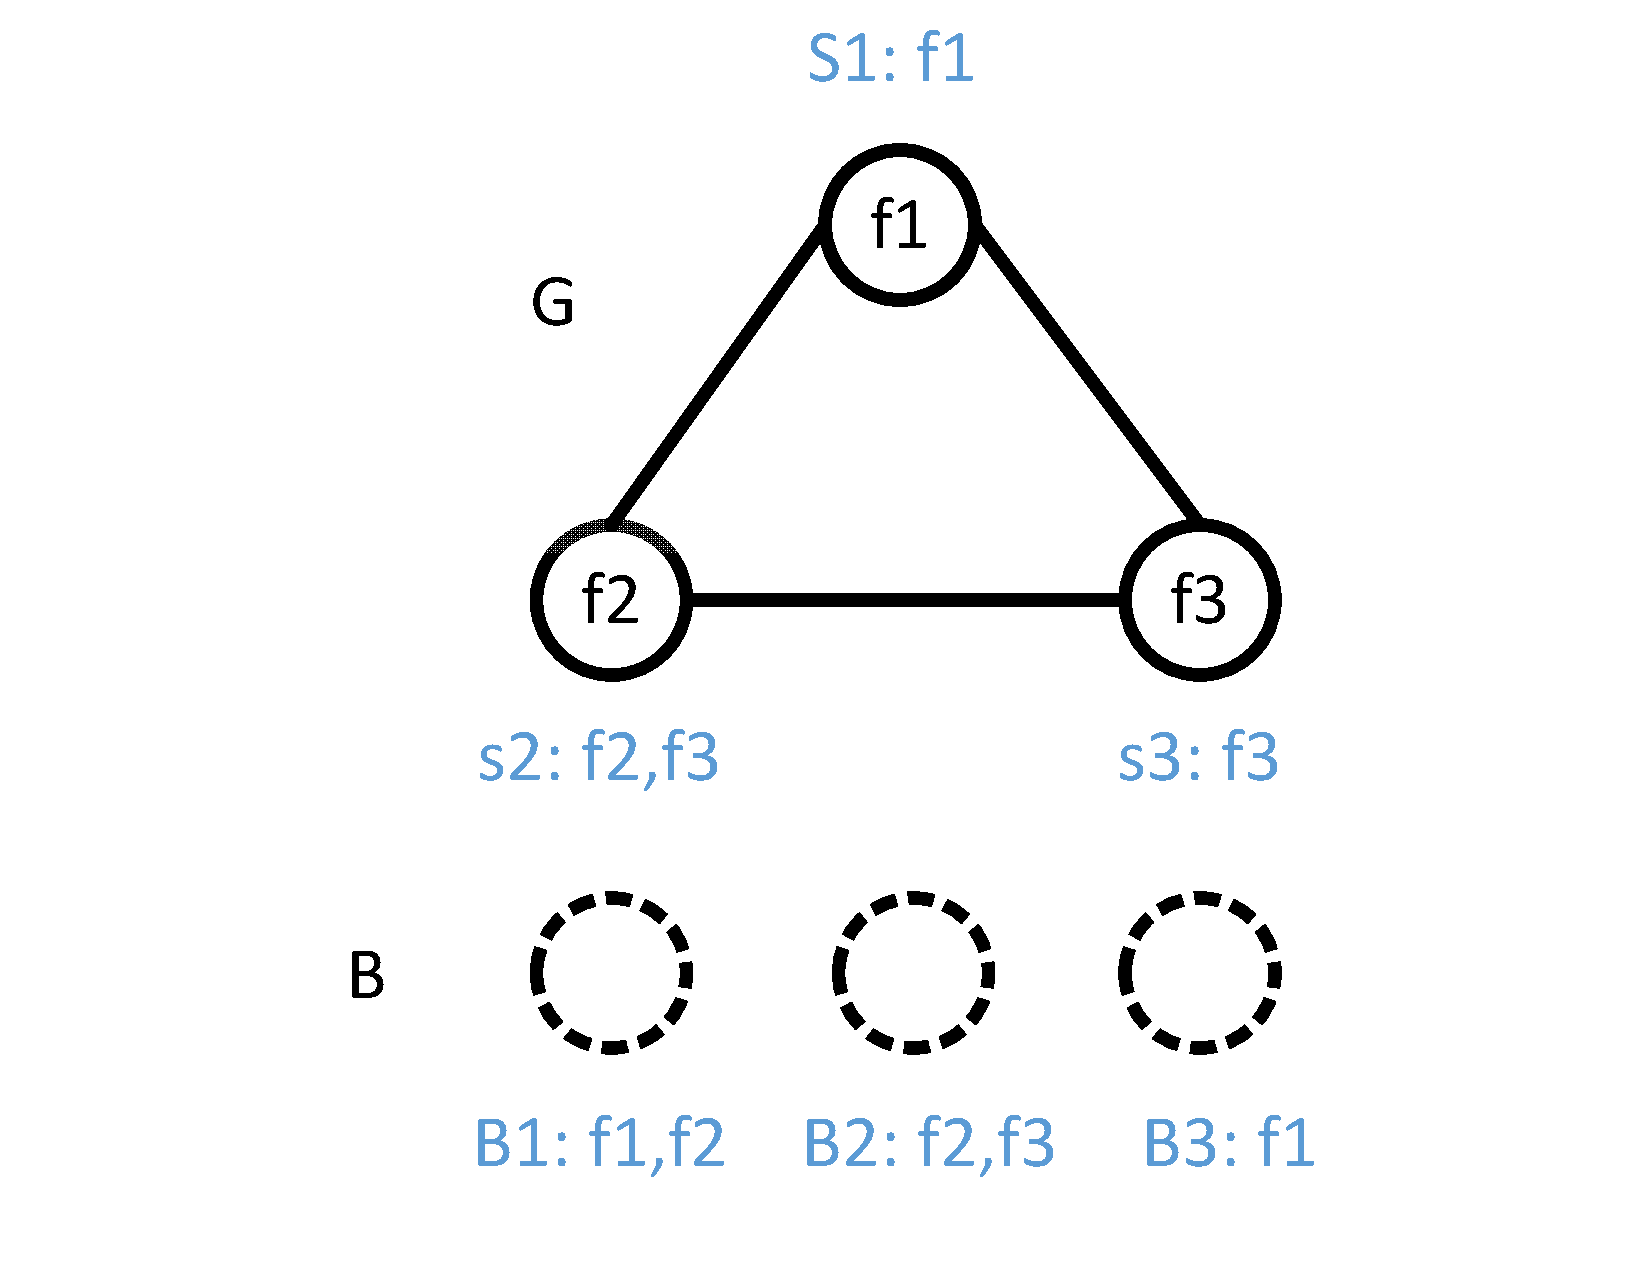
\includegraphics[width=1.5in]{Fig/SNFTBexample}\\
\caption{Graph $G(V,E,S)$: V=$\{v_1,v_2,v_3\}$, E=$\{v_1v_2,v_2v_3,v_3v_1\}$, S=$\{\{s_1\},\{s_2,s_3\},\{s_3\}\}$. Backup node $B(V,S)$: V=$\{b_1,b_2,b_3\}$, S=$\{\{s_1,s_2\},\{s_2,s_3\},\{s_1\}\}$ }\label{fig:SNFTBexample}
\end{minipage}
\hfill
\begin{minipage}[t]{0.3\linewidth}
\centering
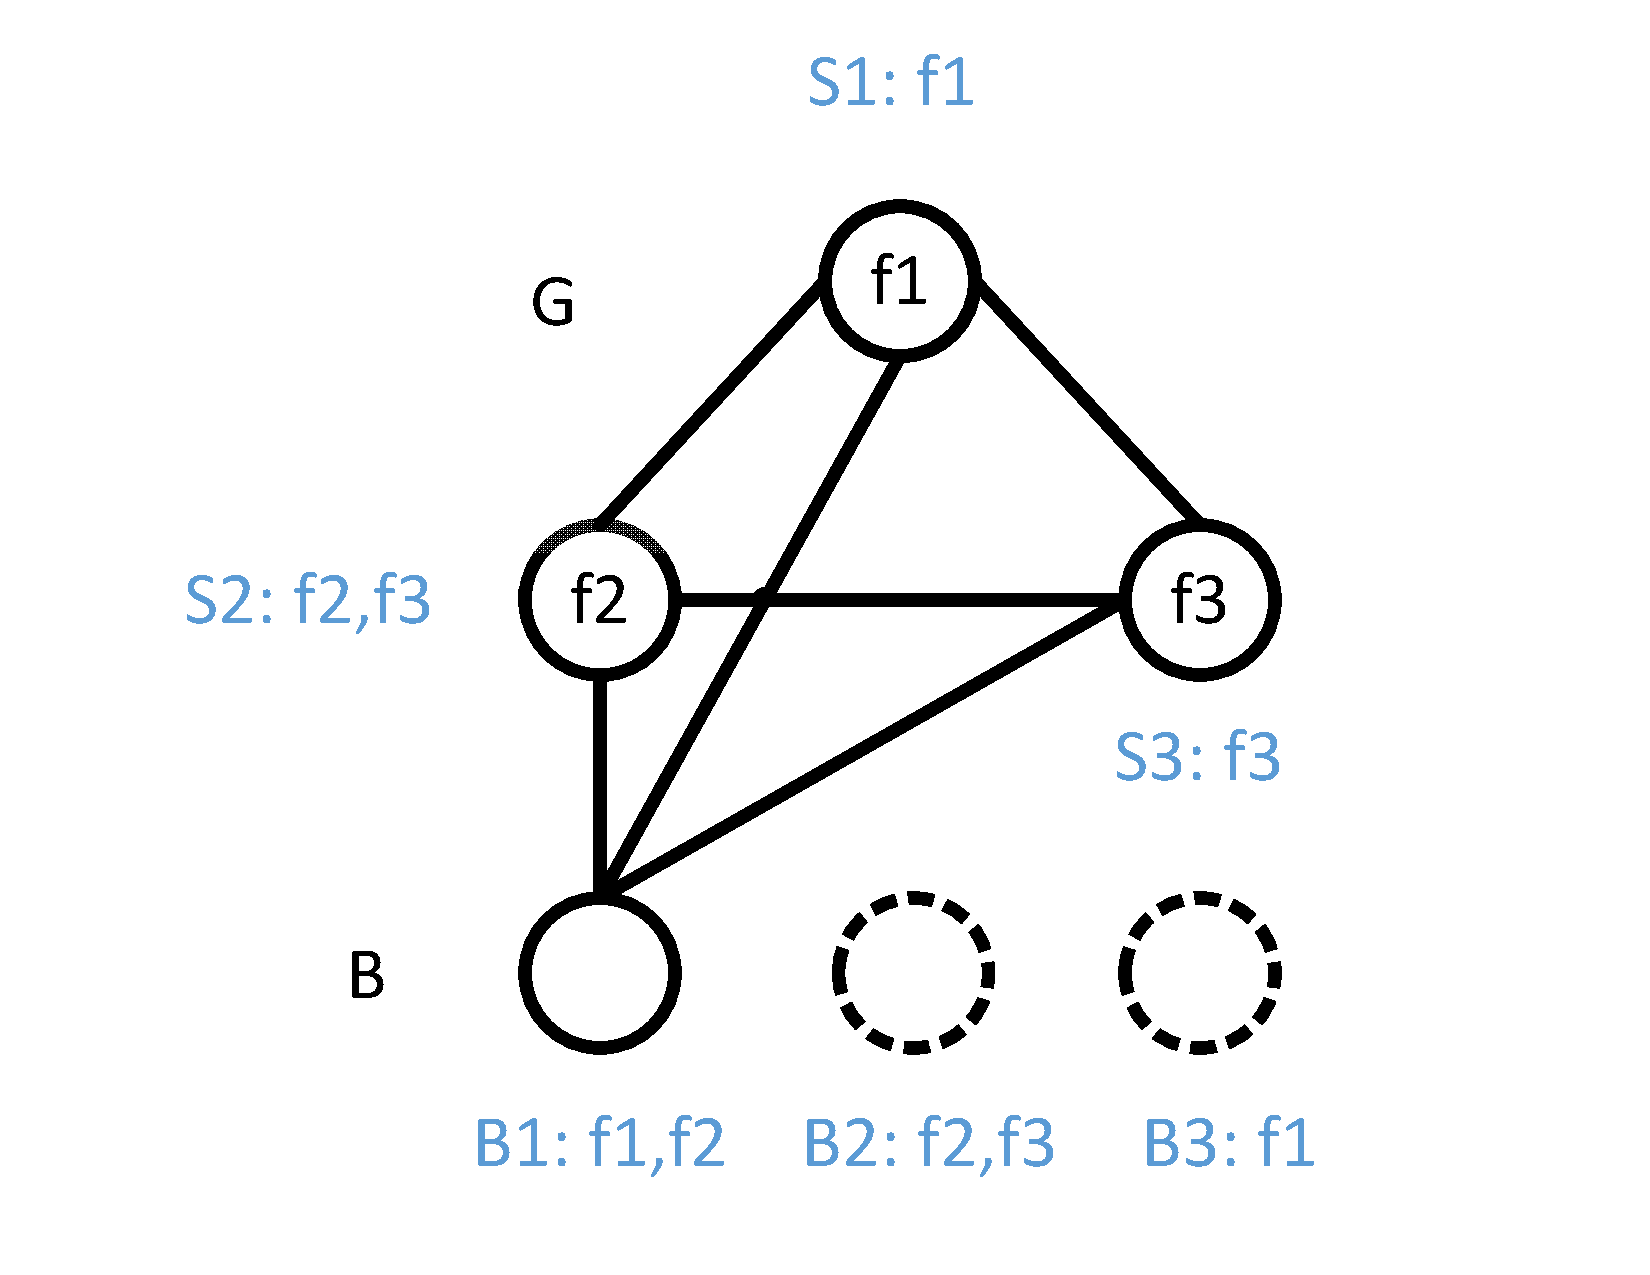
\includegraphics[width=1.5in]{Fig/SNFToptimal}\\
\caption{optimal $1$-SNFT($G(V,E,S),B(V,S)$), $SNFT_{nc}$$(G,1,B)$=1, $SNFT_{ec}$$(G,1,B)$=3.}\label{fig:SNFToptimal}
\end{minipage}
\hfill
\begin{minipage}[t]{0.3\linewidth}
\centering
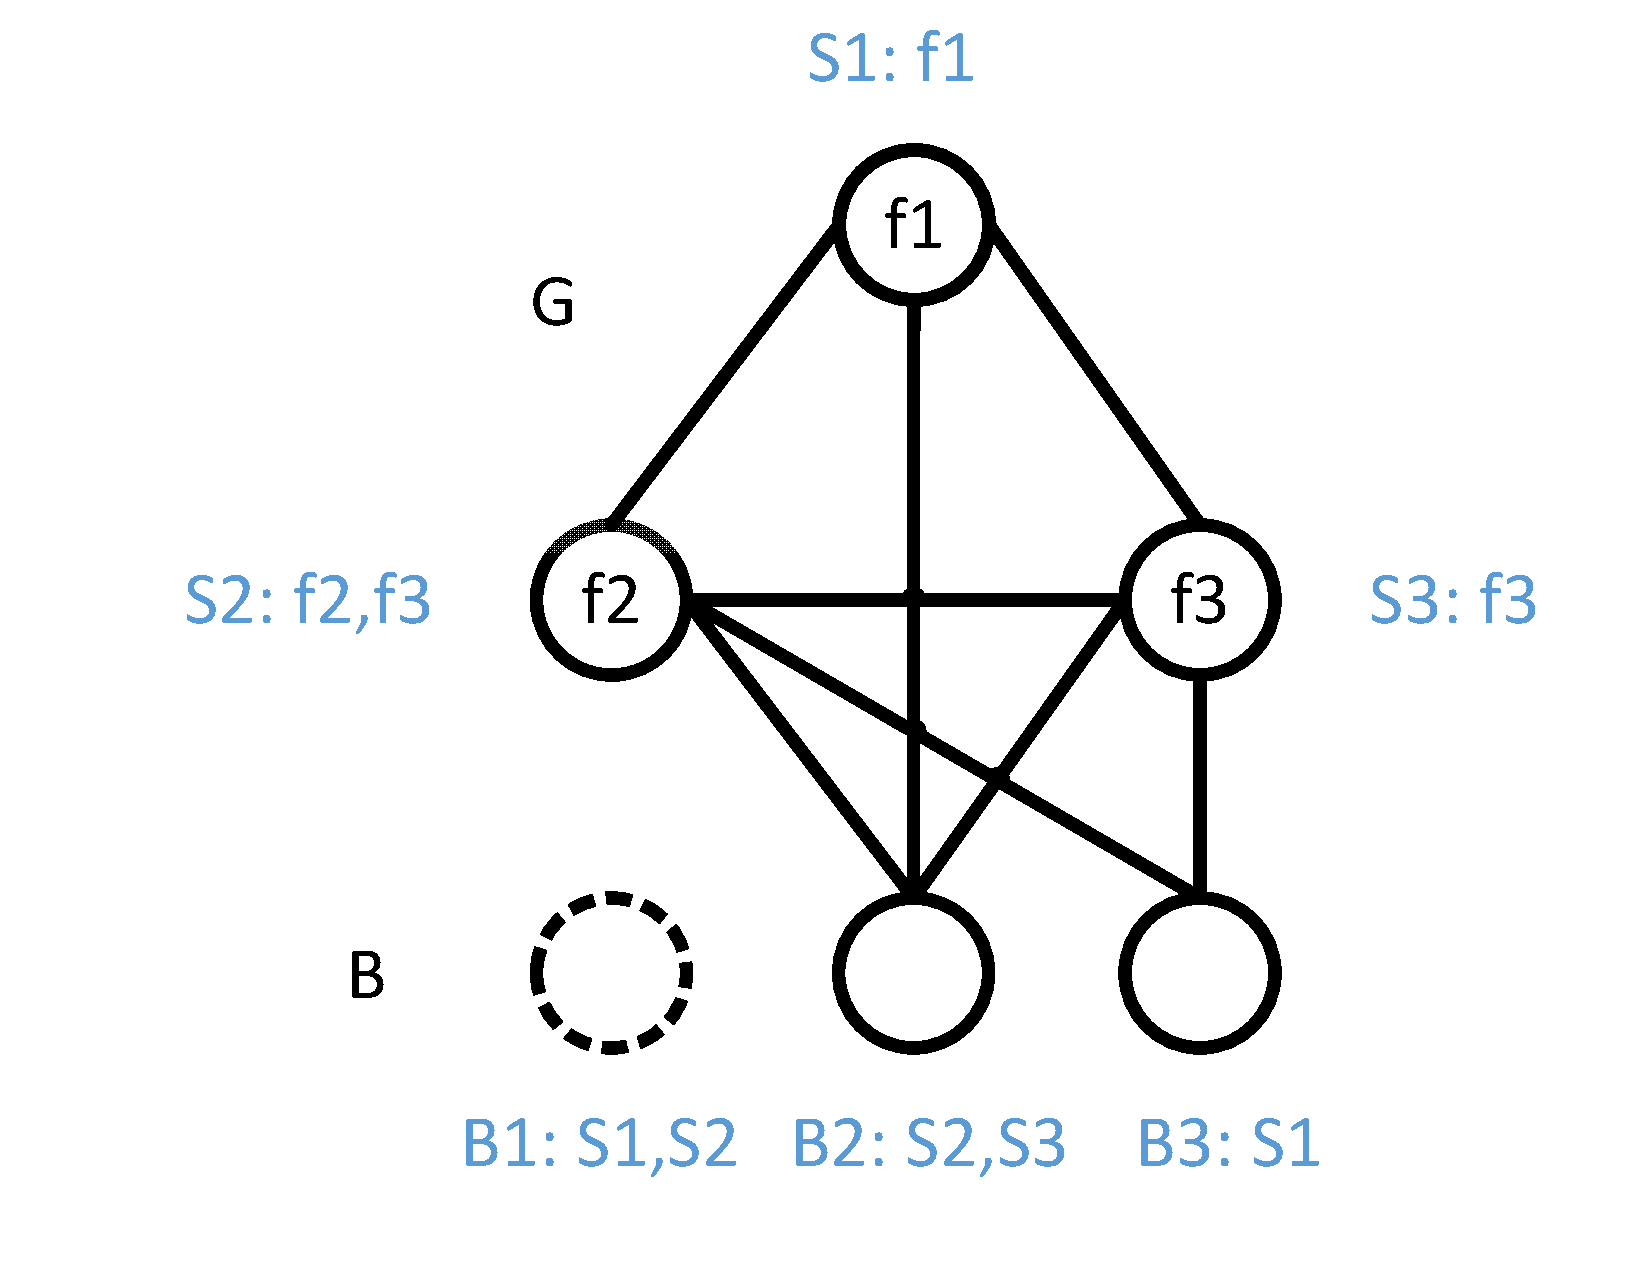
\includegraphics[width=1.5in]{Fig/SNFTnonoptimal}\\
\caption{non optimal $k$-SNFT($G(V,E,S),B(V,S)$), $SNFT_{nc}$$(G,1,B)$=2, $SNFT_{ec}$$(G,1,B)$=5}\label{fig:SNFTnonoptimal}
\end{minipage}
\end{figure*}


\begin{figure*}[tp]
\centering
\begin{minipage}[t]{0.3\linewidth}
\centering
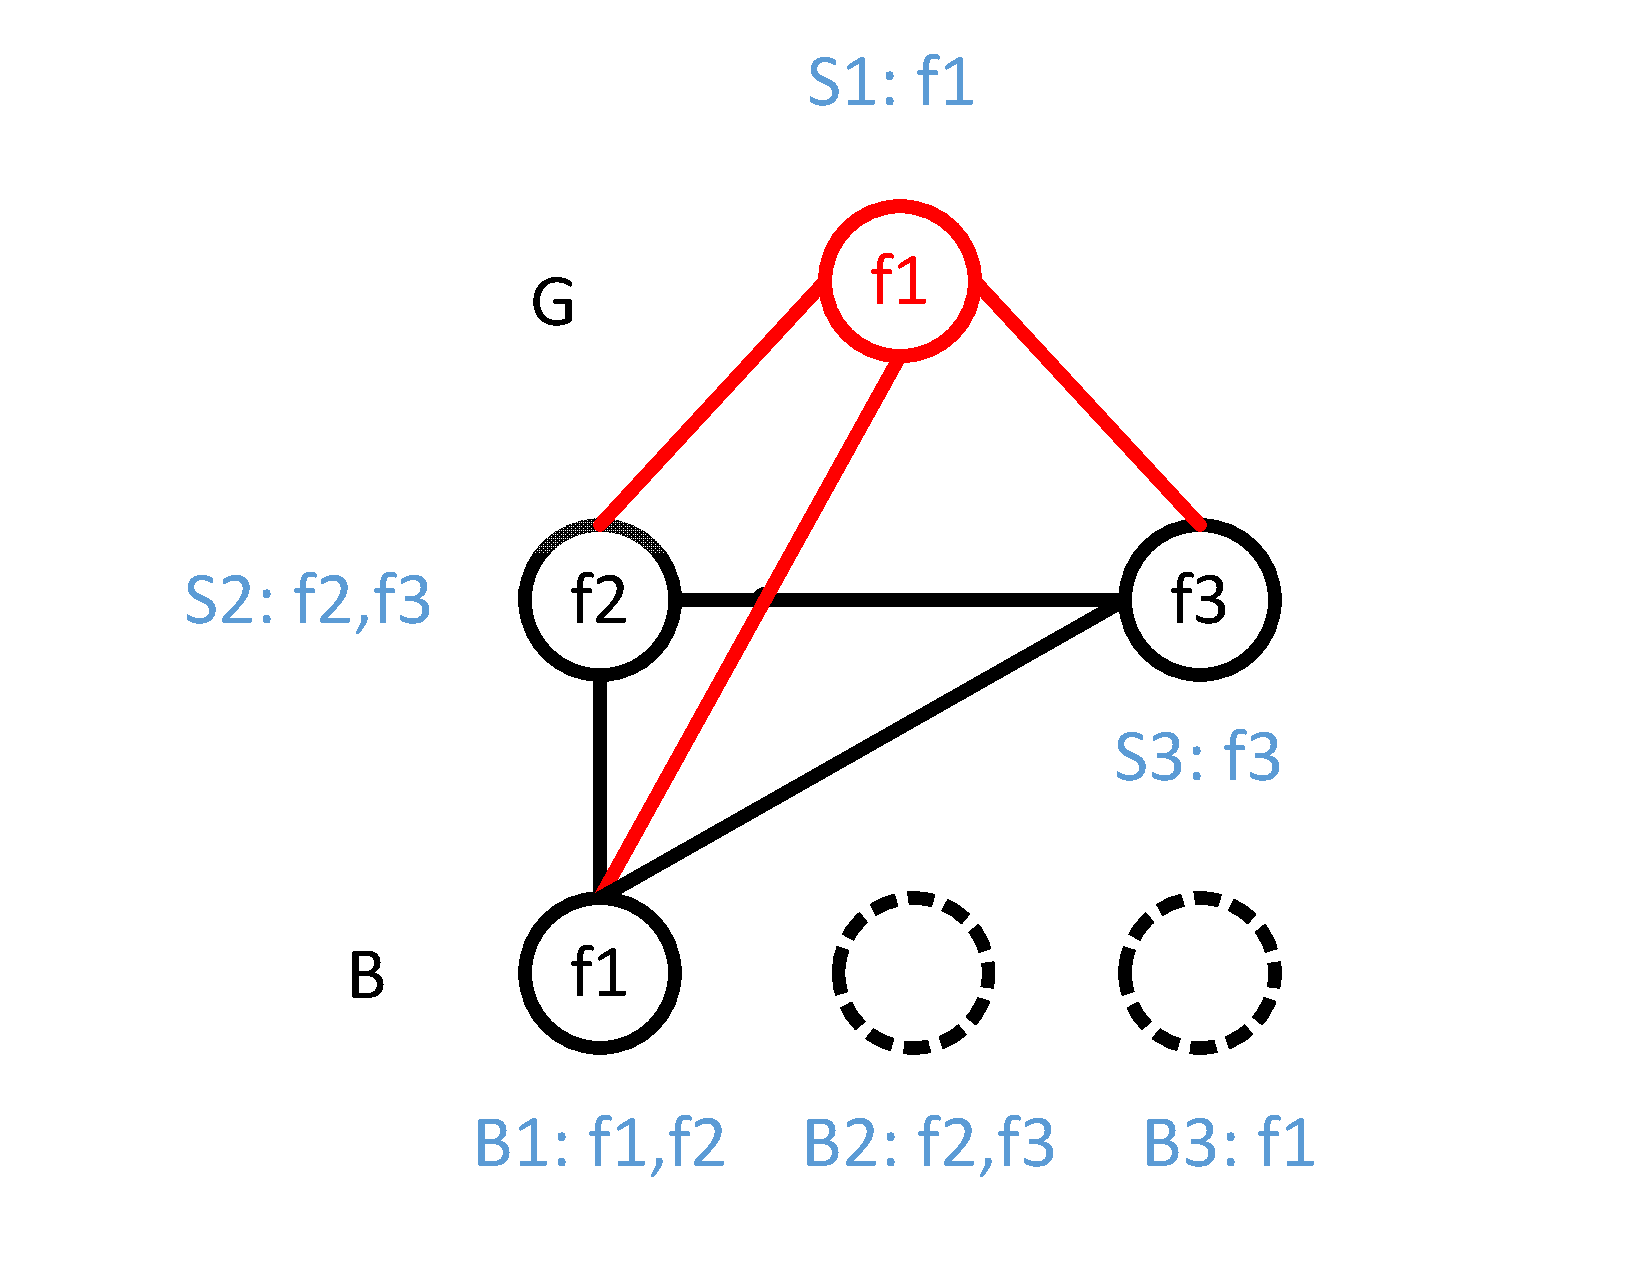
\includegraphics[width=1.5in]{Fig/SNFToptimal_n1Fail}\\
\caption{optimal $k$-SNFT($G(V,E,S),B(V,S)$) when node $v_1$ fail, node $v_1$ transform to $b_1$}\label{fig:SNFToptimal_n1Fail}
\end{minipage}
\hfill
\begin{minipage}[t]{0.3\linewidth}
\centering
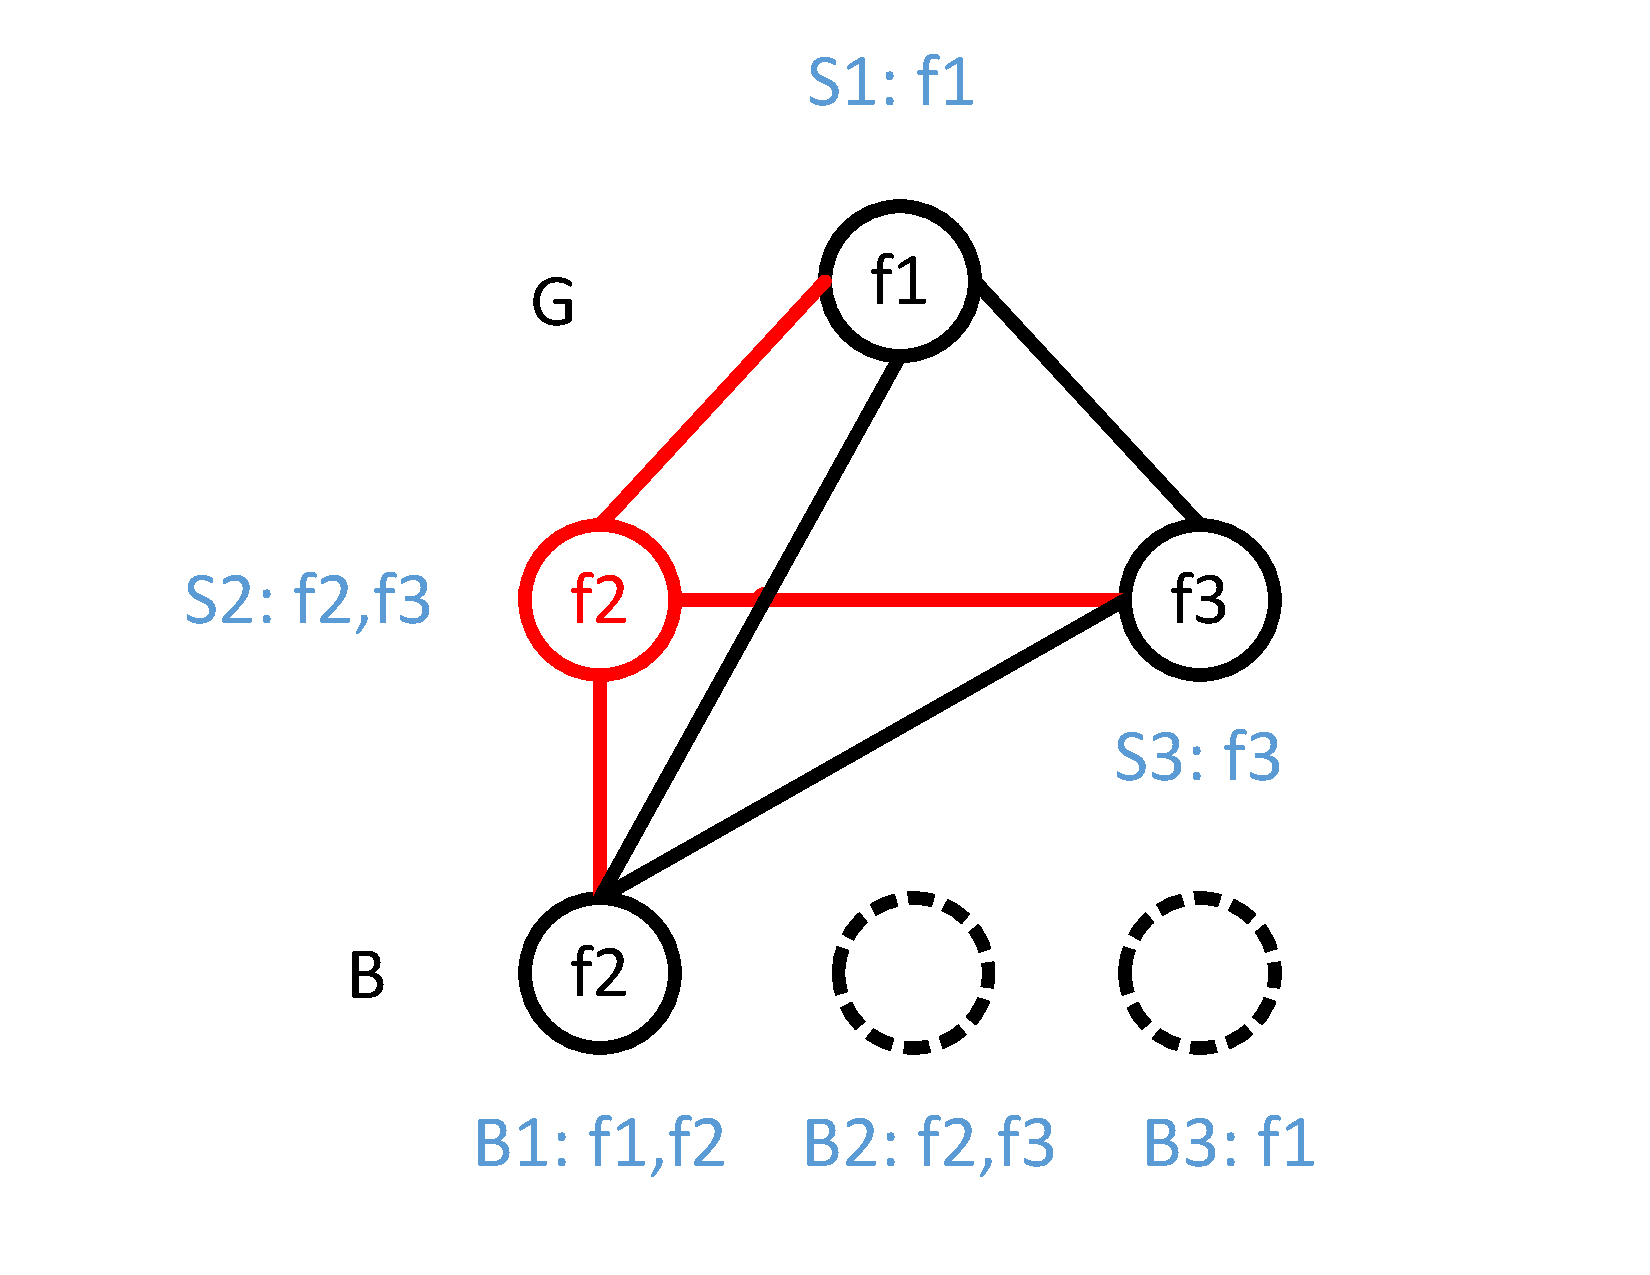
\includegraphics[width=1.5in]{Fig/SNFToptimal_n2Fail}\\
\caption{optimal $k$-SNFT($G(V,E,S),B(V,S)$) node $v_2$ fail, node $v_2$ transform to $b_1$}\label{fig:SNFToptimal_n2Fail}
\end{minipage}
\hfill
\begin{minipage}[t]{0.3\linewidth}
\centering
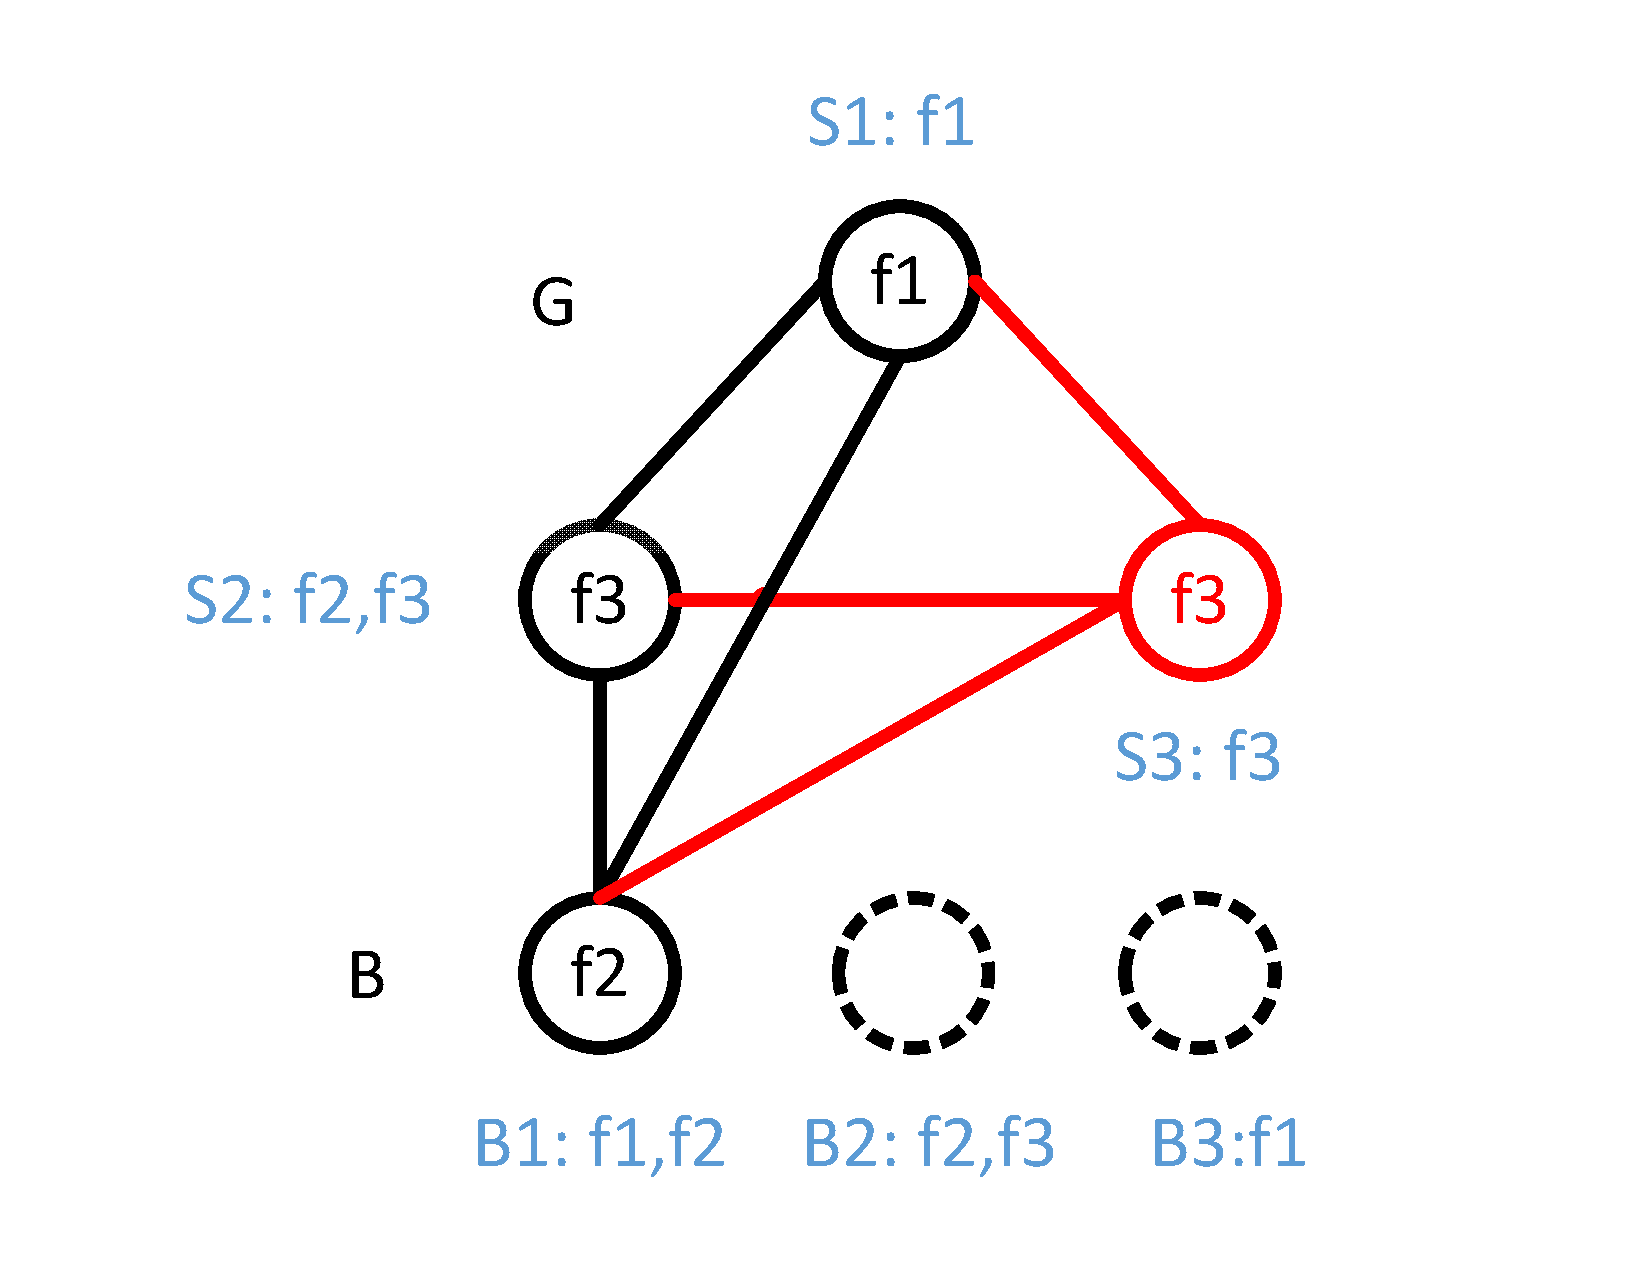
\includegraphics[width=1.5in]{Fig/SNFToptimal_n3Fail}\\
\caption{optimal $k$-SNFT($G(V,E,S),B(V,S)$) node $v_3$ fail, node $v_2$ transform to $b_1$, node $v_3$ transform to $v_2$}\label{fig:SNFToptimal_n3Fail}
\end{minipage}
\end{figure*}


Generally speaking, survivable embedded virtual network's request is 1-service node fault-tolerant of virtual network $G(V,E,S,L)$ with backup nodes set $B(V,S)$. Inserting any edges among nodes $V\cup B$ to construct $G^o$ as shown in Fig.\ref{fig:FI},\ref{fig:FD}, for which G is a subgraph of $G^o-v(\forall v\in V\cup B^o,B^o\subset B)$.

%$G^o$([1-SNFT(G),B]) is survivable virtual network $SVN$.(one node of backup nodes n failed, )
We would link some edges amongst nodes $V\cup B$ to construct 1-SNFT graph of arbitrary graph $G$ as show Fig.\ref{fig:FI},\ref{fig:FD}, when only one node of VN failed, the former graph of VN is also subgraph isomorphism of graph of SVN. %For example, when node v3 failed the node v2 run service 3 and backup node run service 2 so that the graph of VNR is subgraph isomorphism of SVN-v3 as shown in figure \ref{fig:optgraph_n1_fail},\ref{fig:optgraph_n2_fail},\ref{fig:optgraph_n3_fail}, the red edge and red node is disable.




\subsection{After node failure reducing immigration}
However, this poses a limitation since the result only guarantees graph isomorphism and not equality. In other words, there may be a need to physically swap remaining VMs while recovering from some failure in order to return to the original infrastructure G. Recovery may then be delayed, or require more resources for such swapping operations.





%write the bandwith and computting resource between FI and FD.
\begin{figure}
\centering
% Requires \usepackage{graphicx}
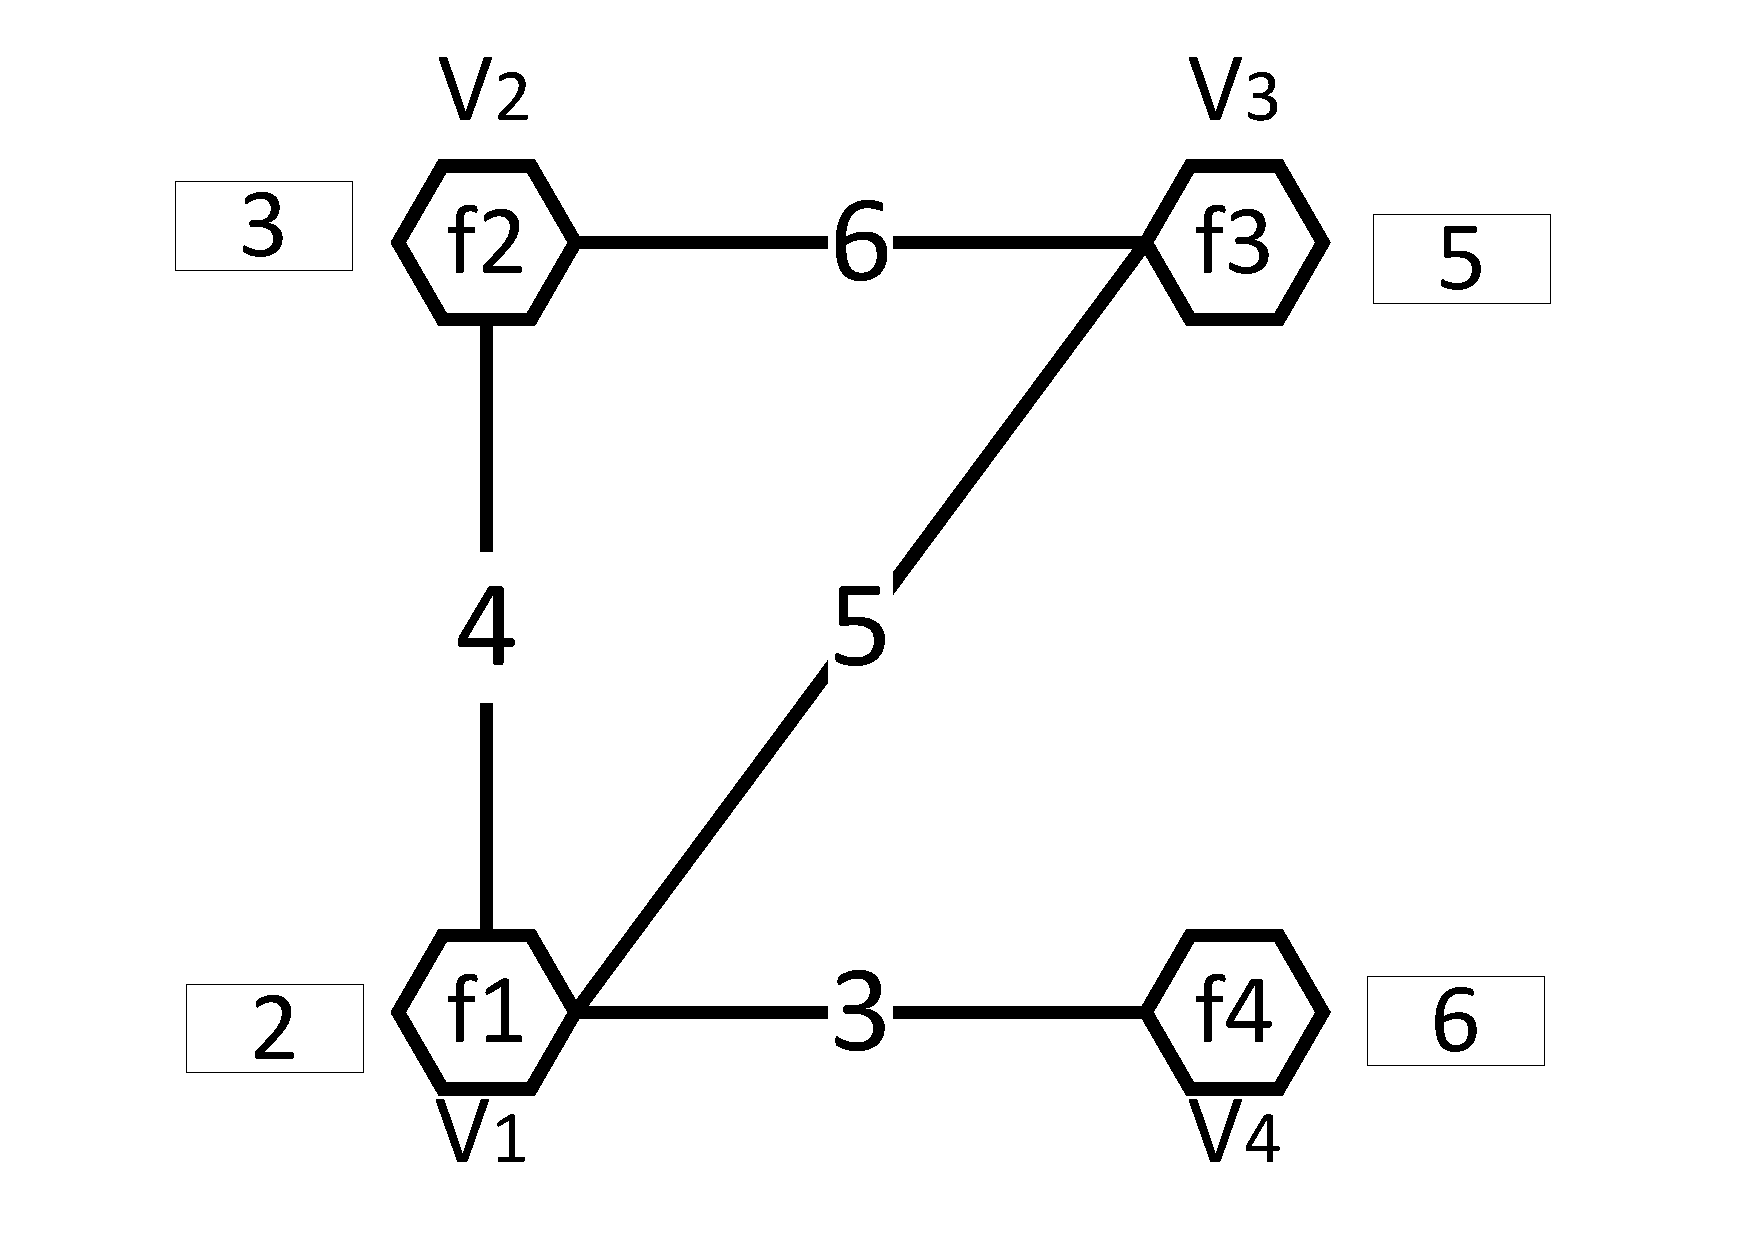
\includegraphics[width=2in]{Fig/VNQ}\\
\caption{Virtual Network Request: $G^V (V^V,E^V,s^V,L^V)$}\label{fig:VNQ}
\end{figure}

\begin{figure}
\centering
% Requires \usepackage{graphicx}
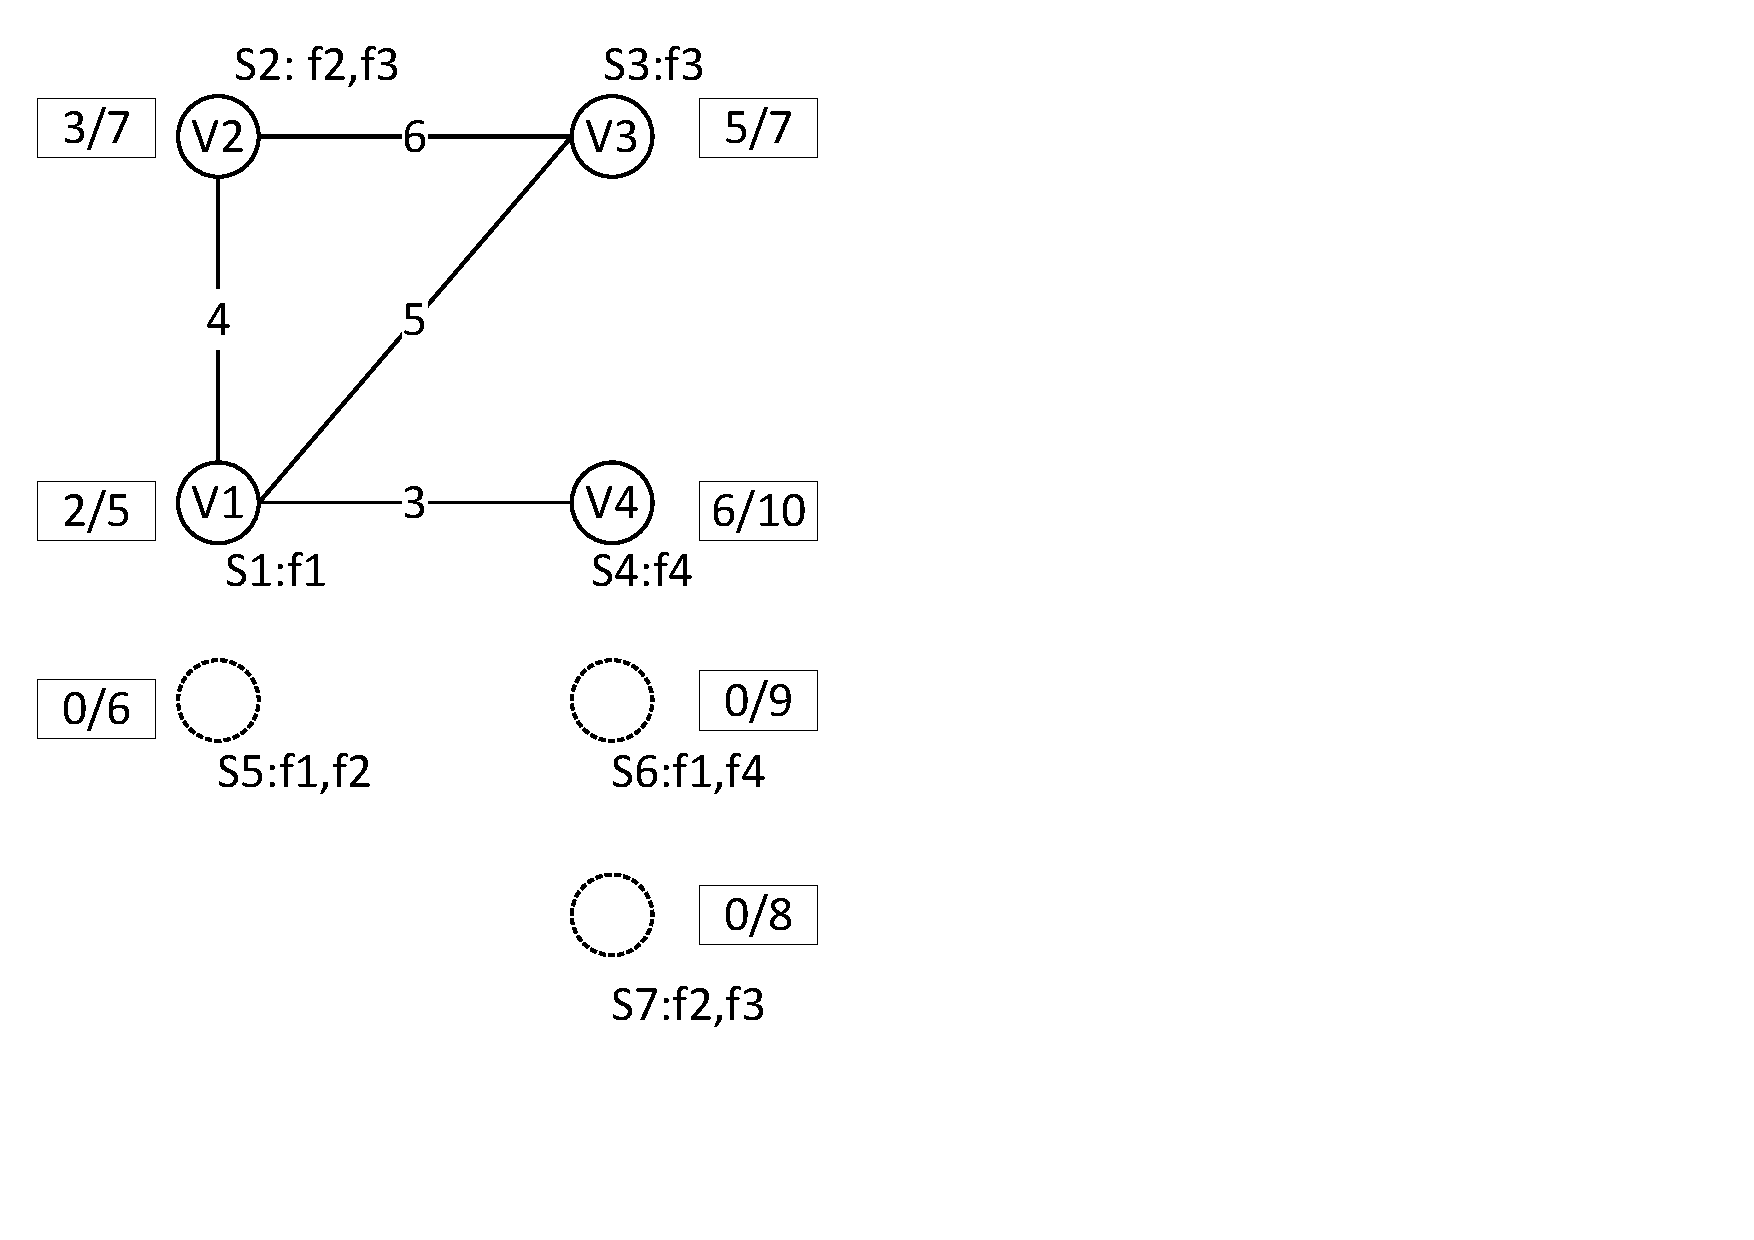
\includegraphics[width=2in]{Fig/eVN}\\
\caption{embedded Virtual Network: $G^V (V^V,E^V,s^V,L^V,S^V,C^V,B^V,M^V_V)$}\label{fig:eVN}
\end{figure}

\begin{figure}
\centering
\begin{minipage}[t]{0.5\linewidth}
\centering
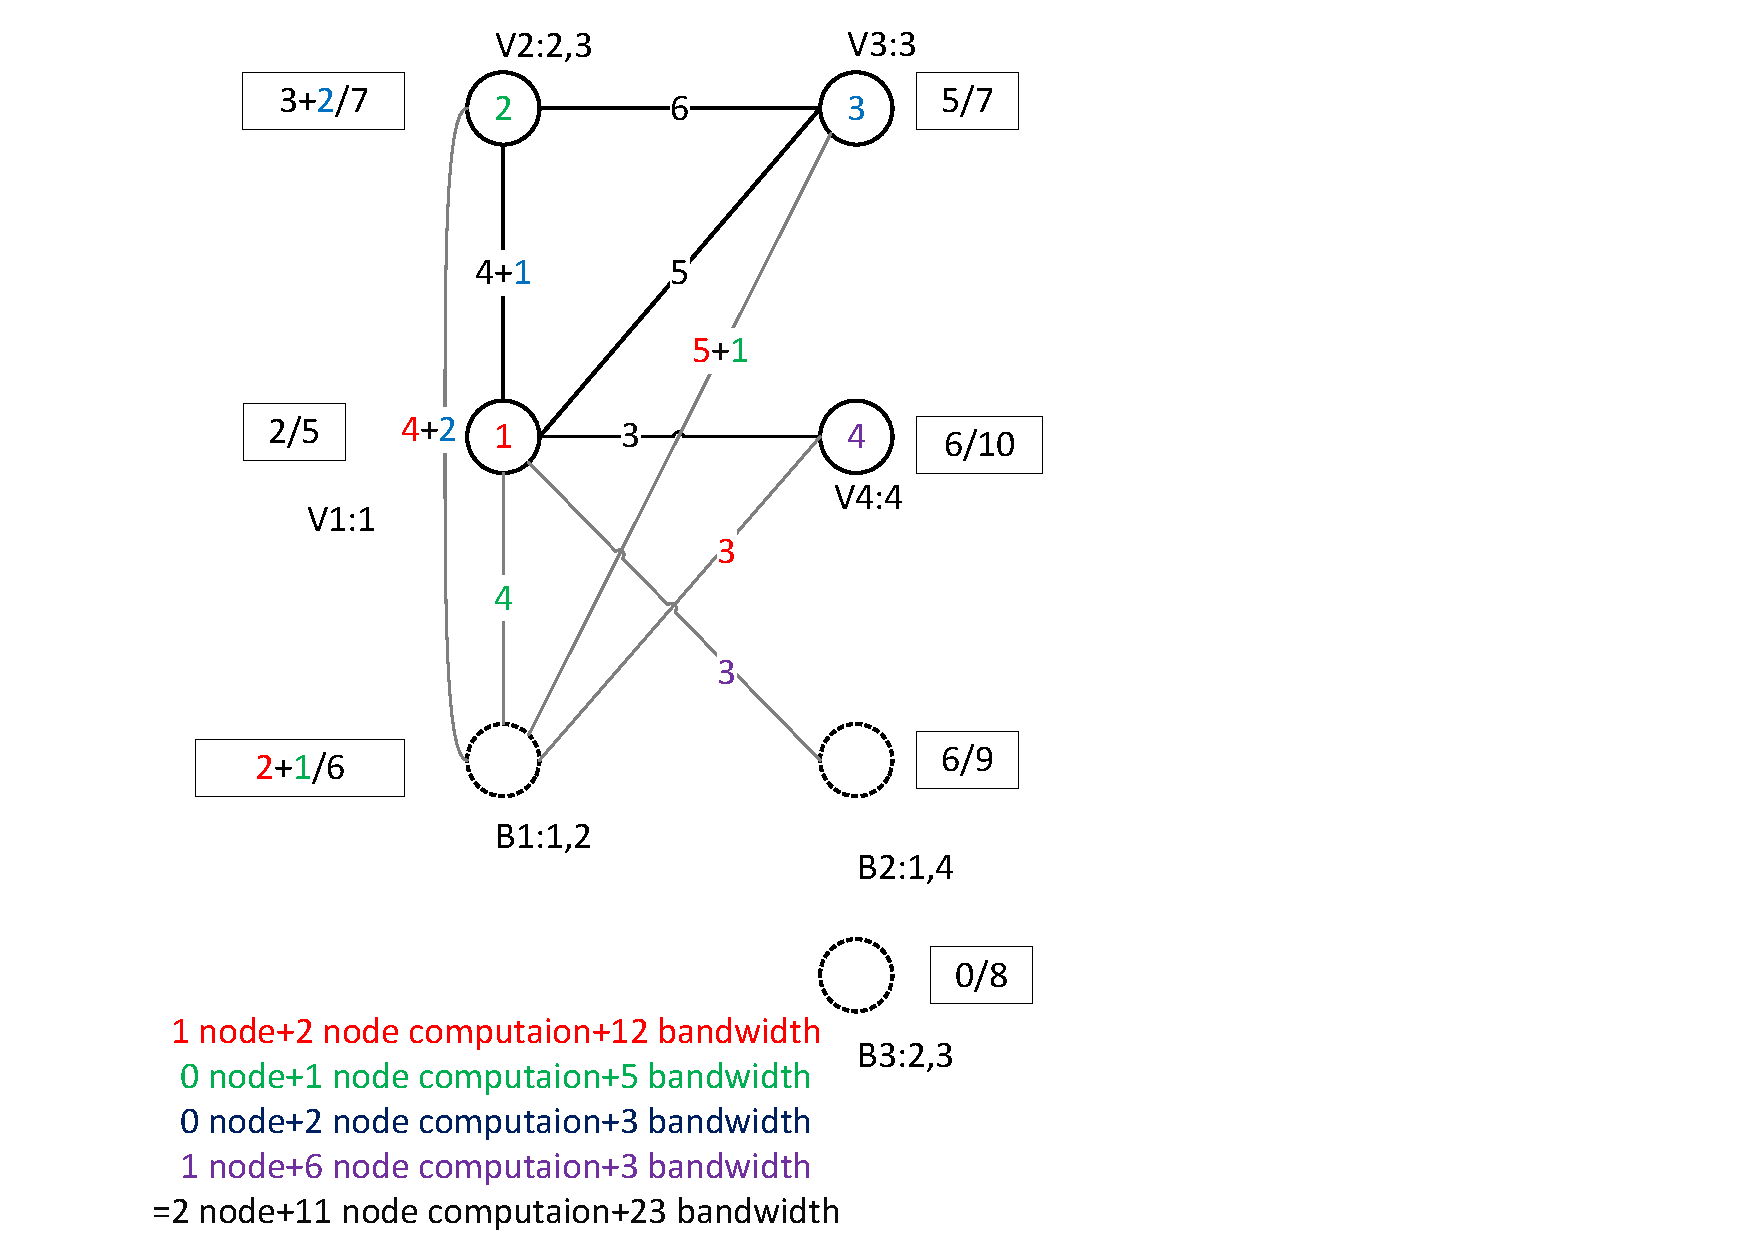
\includegraphics[width=1in]{Fig/FD}\\
\caption{ FD}\label{fig:FD}
\end{minipage}
\hfill
\begin{minipage}[t]{0.5\linewidth}
\centering
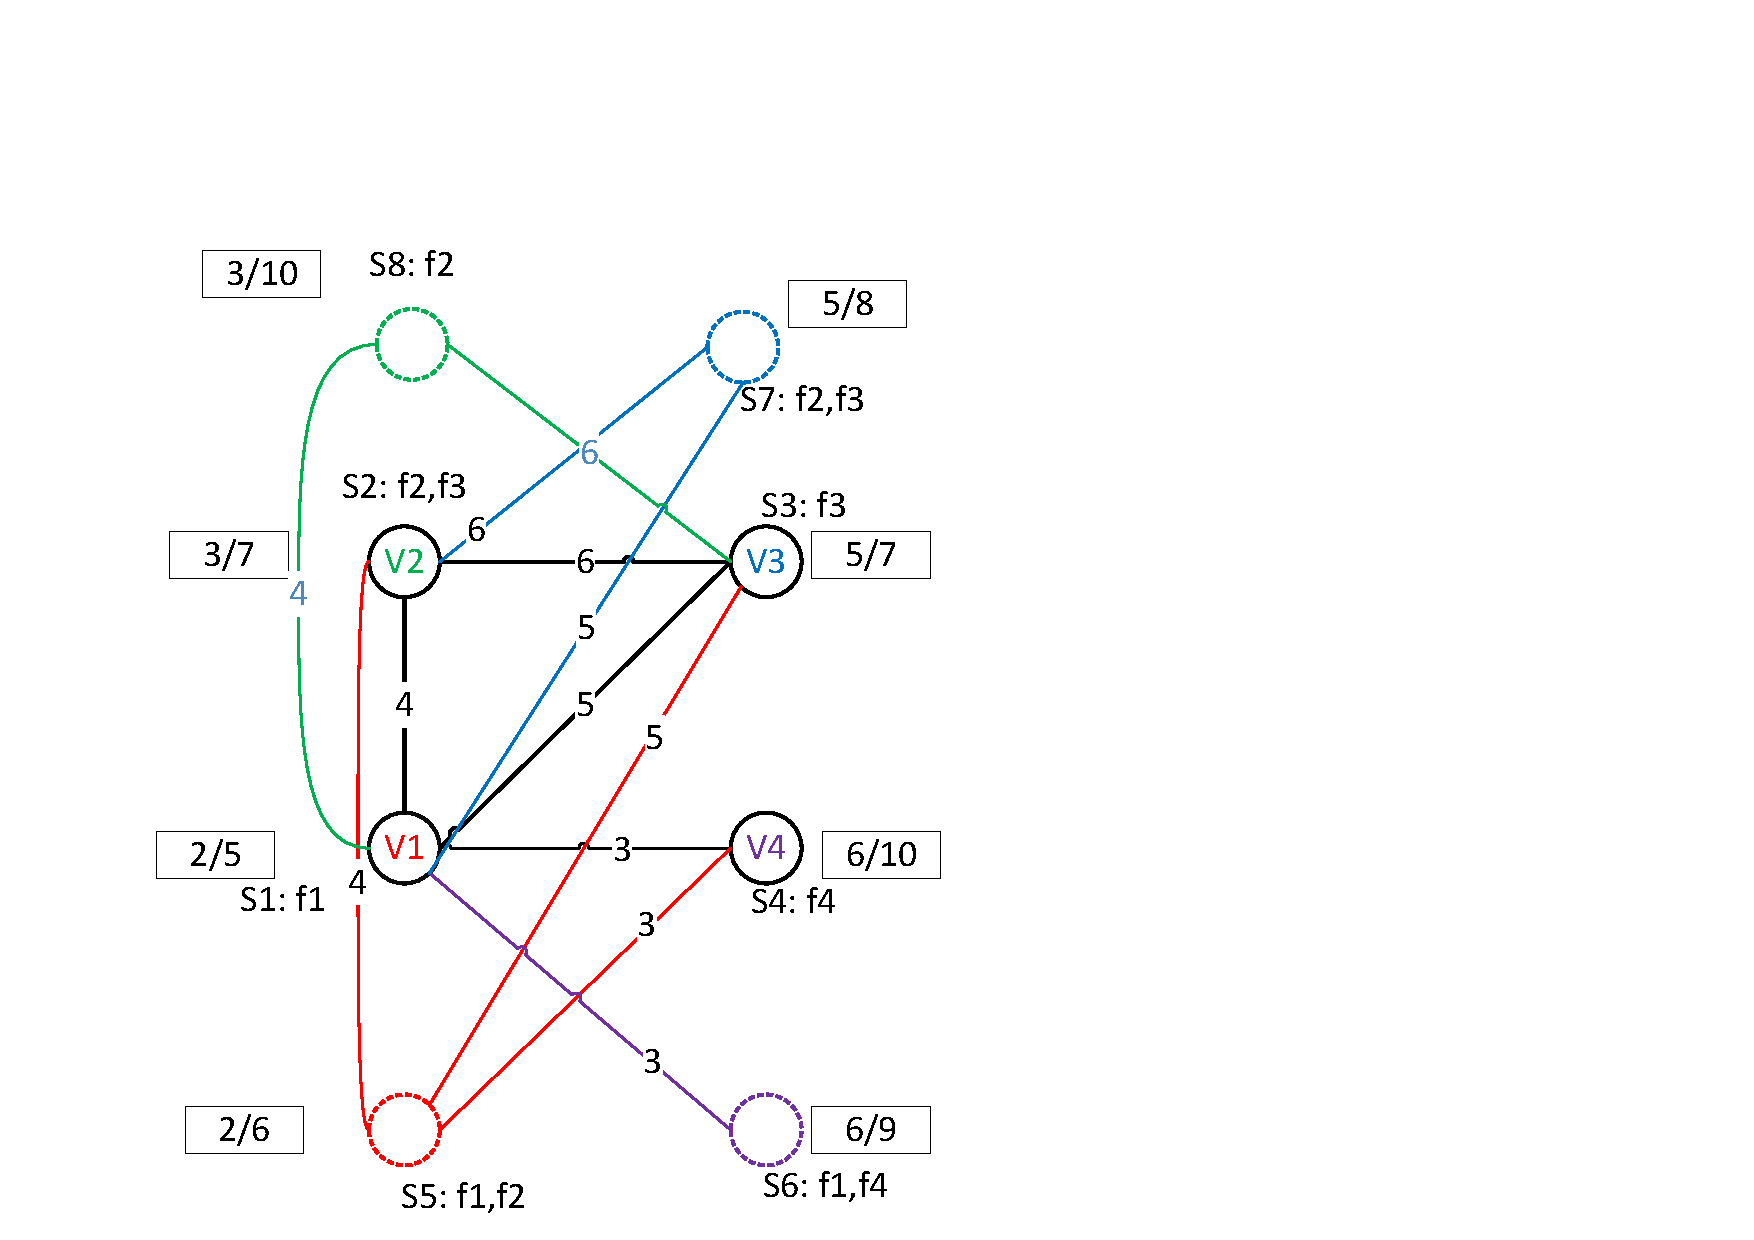
\includegraphics[width=1in]{Fig/FI}\\
\caption{FI}\label{fig:FI}
\end{minipage}
\end{figure}




